\documentclass{article}
\usepackage{amsmath,amssymb,amsthm,mdframed,kotex,paralist}
\usepackage{tabto}
%\TabPositions{0.5\textwidth}
\TabPositions{0.33\textwidth,0.66\textwidth}
\newcommand\bp[1]{\begin{mdframed}[frametitle={#1},skipabove=10pt,skipbelow=20pt,innertopmargin=5pt,innerbottommargin=40pt]}
\newcommand\ep{\end{mdframed}\par}
\newcommand\ov[1]{\ensuremath{\overline{#1}}}

\begin{document}
\title{연습문제들(중학교1학년--고등학교1학년)}
\author{}
\date{\today}
\maketitle

\section{인수분해와 전개}
\bp{01}
다음 수들을 간단히 하시오.
\begin{enumerate}[(1)]
\item
\((\sqrt2)^4\)
\item
\(\sqrt 8+\sqrt{18}\)
\item
\((\frac{3^3}{3^2})^3+(\frac{2^2}{2^3})^2\)
\item
\(\frac{5}{\sqrt3}\)
\item
\(\frac{4}{2-\sqrt3}\)
\end{enumerate}
\ep

\bp{02}
다음을 전개 하시오.
\begin{enumerate}[(1)]
\item
\((a+b)^2\)
\item
\((t+2)^2\)
\item
\((2x+y)(x+2y)\)
\item
\((a+b+c)^2\)
\end{enumerate}
\ep

\bp{03}
다음을 인수분해 하시오.
\begin{enumerate}[(1)]
\item
\(x^2-2xy+y^2\)
\item
\(a^2-b^2\)
\item
\(t^2-t-2\)
\item
\(x^3-2x+1\)
\end{enumerate}
\ep

\bp{04}
다음 방정식을 푸시오(단 \(x\)는 실수).
\begin{enumerate}[(1)]
\item
\(2x-4=0\)
\item
\(\frac12x+3=0\)
\item
\(x^2-3x-4=0\)
\item
\(2x^2+5x-3=0\)
\end{enumerate}
\ep

\bp{05}
다음 연립방정식을 푸시오.
\begin{enumerate}[(1)]
\item
\(\left\{\begin{array}{c}
3x+y=5\\
x+y=1
\end{array}\right.\)
\item
\(\left\{\begin{array}{c}
a^2+b^2=25\\
ab=12
\end{array}\right.\)
\item
\(\left\{\begin{array}{c}
x^2-xy-2y^2=0\\
x^2+2xy-3y^2=20
\end{array}\right.\)
\end{enumerate}
\ep

\bp{06}
다음 삼각비의 값을 구하시오.
\begin{enumerate}[(1)]
\item
\(\sin 60^\circ\)
\item
\(\cos 90^\circ\)
\item
\(\tan 150^\circ\)
\item
\(\sin\frac\pi6\)
\item
\(\sec(-\frac56\pi)\)
\end{enumerate}
\ep

\bp{07}
전체집합 \(U=\{1,2,\cdots,10\}\)의 두 부분집합 \(A=\{x\;|\;x\text{는 3의 배수}\}\), \(B=\{x\;|\;x\text{는 4의 배수}\}\)에 대하여 다음을 원소나열법으로 나타내어라.
\begin{enumerate}[(1)]
\item
\(A\cap B\)
\item
\(A\cup B\)
\item
\(A-B\)
\item
\(A^c\cap B^c\)
\end{enumerate}
\ep

\bp{08}
다음 주어진 도형에서 \(\overline{BC}\)의 길이를 구하여라.
\par\center
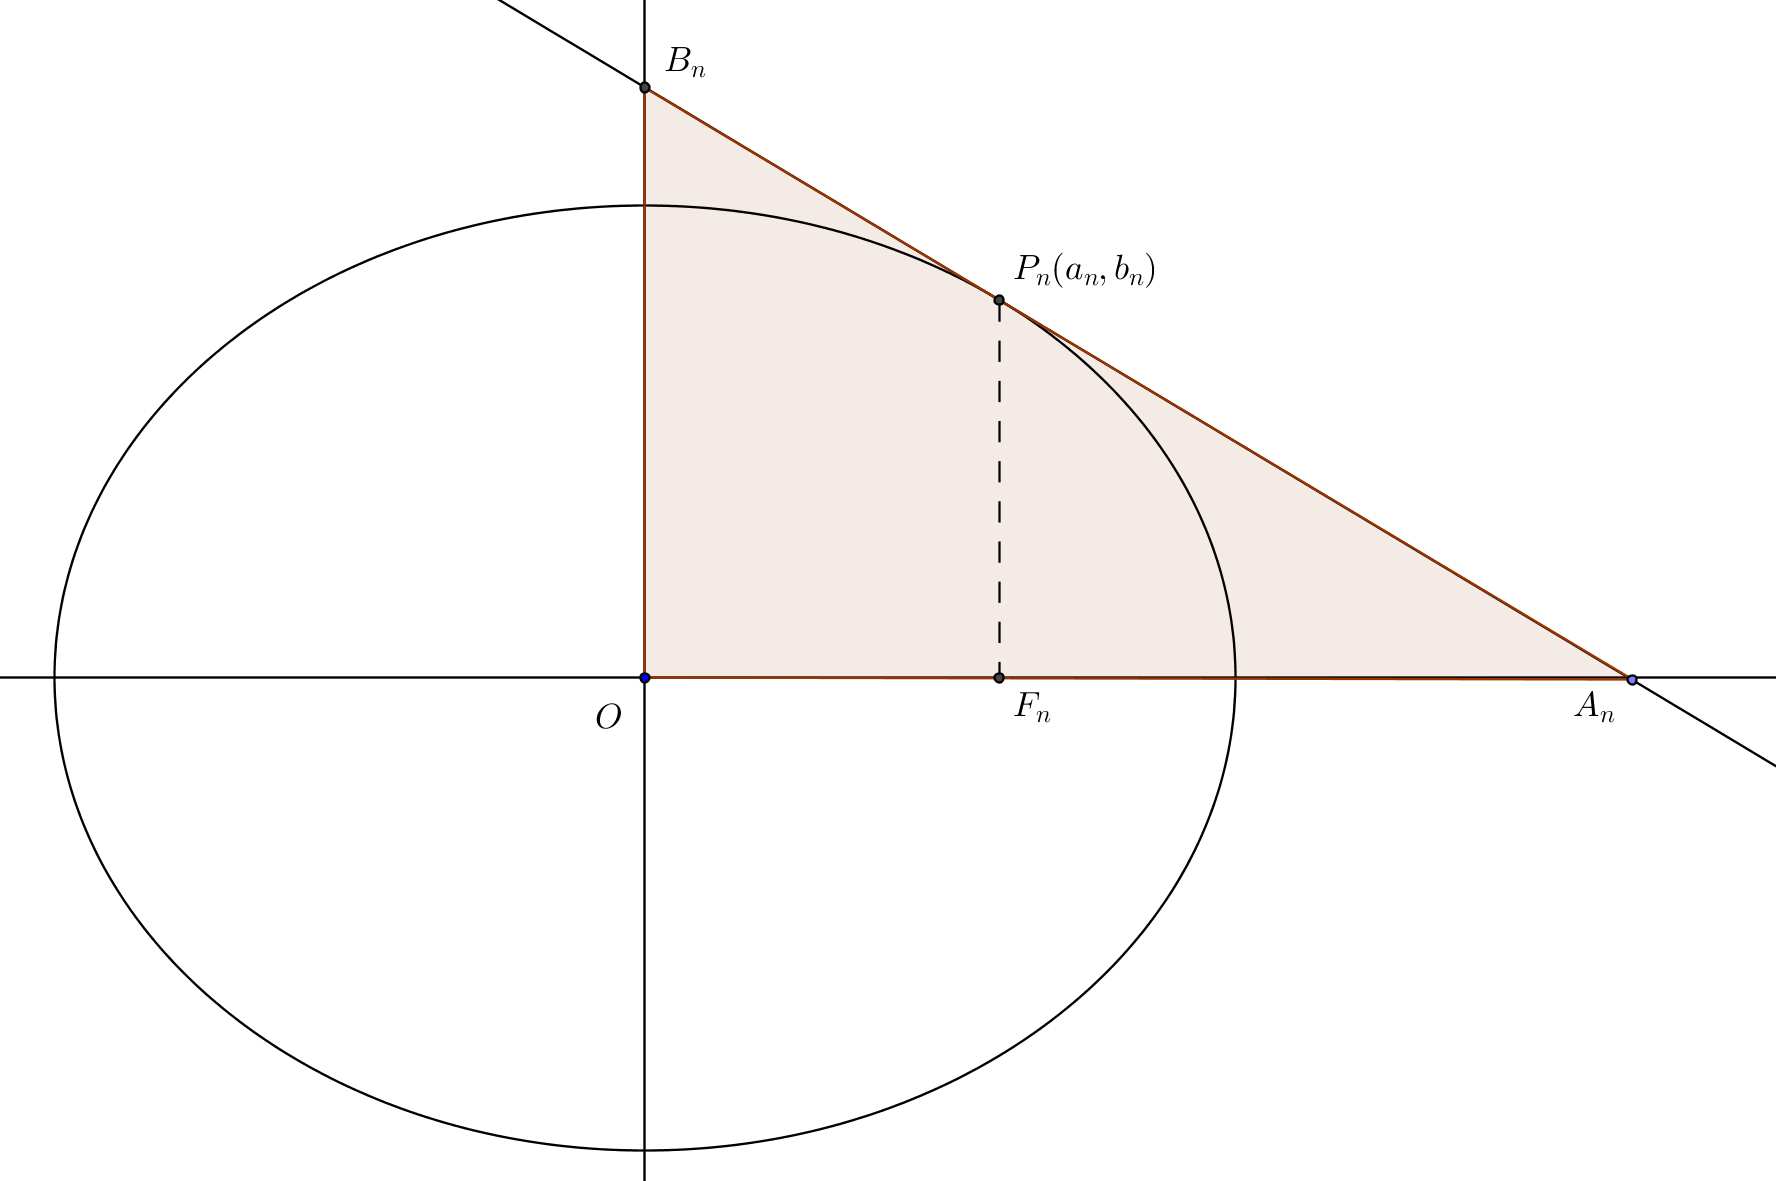
\includegraphics[width=0.3\textwidth]{01}
\ep

\bp{09}
다음 주어진 도형에서 \(\overline{AB}\)의 길이를 구하여라.
\par\center
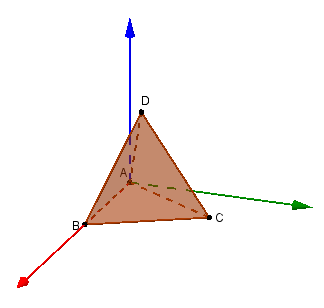
\includegraphics[width=0.7\textwidth]{02}
\ep

\bp{10}
다음 주어진 도형에서 \(\triangle ABC\)의 넓이를 구하여라.
\par\center
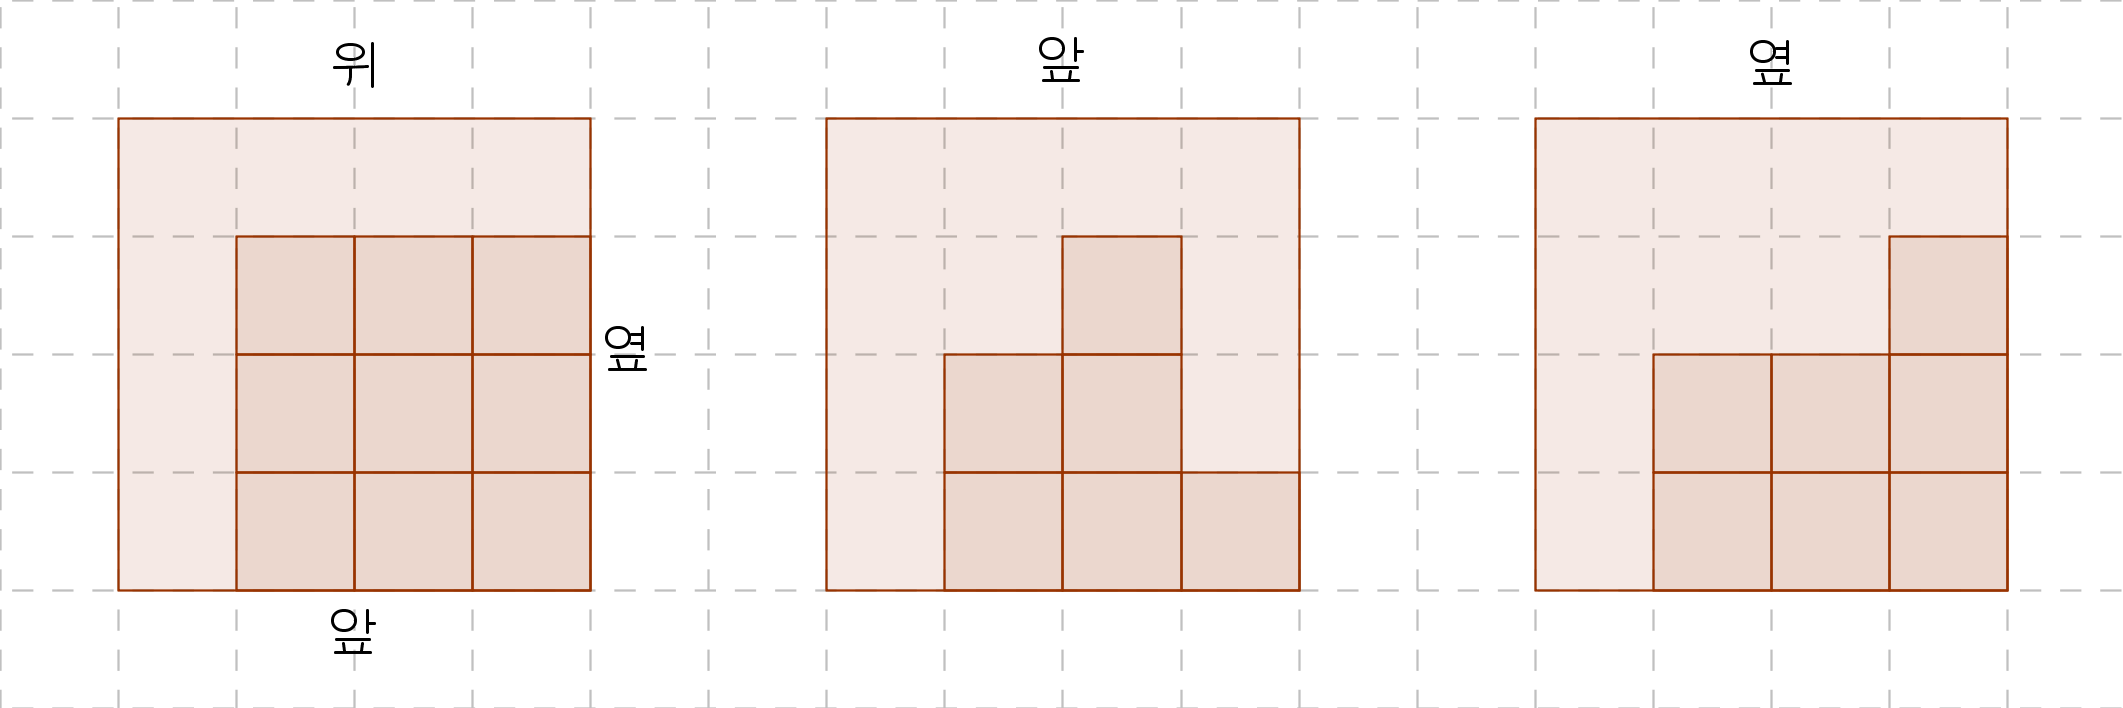
\includegraphics[width=0.6\textwidth]{03}
\ep


\end{document}